\begingroup
\raggedbottom
\setlength{\textfloatsep}{12pt}
\setlength{\intextsep}{12pt}
\renewcommand{\resstep}[1]{\par\smallskip\noindent\QualificationSection{#1}\par\nobreak\smallskip}
\label{sec:results}
The six qualification tests follow the Project Proposal. Tables and figures give the measurements, while Section~\ref{sec:discussion} discusses their engineering meaning. Each test points to supporting evidence in Appendix~\ref{app:res-evidence}.

\subsection{Summary of results achieved}
\label{sec:res-summary}
Table~\ref{tab:res-summary} summarises the measured outcomes. Geometric agreement relative to natural writing is reported separately from character accuracy.
\begin{table}[H]\centering\small
\begin{tabularx}{\linewidth}{p{.25\linewidth}X}\toprule
Requirement & Recorded result\\\midrule
R1. Reproduce text and retain writer style & Reader score on physical output 84.41\%. Writer identification 86.41\% of lines and 14/14 page pools. Normalised geometric agreement 86.68\% on the repeated-word subset.\\[3pt]
R2. At least 95\% text and writer accuracy & Reader 94.06\%. Writer identification 153/156 lines (98.08\%).\\[3pt]
R3. At most 4 s per reproduced character & All 25 completed ODROID requests pass. Largest recorded value 3.875 s per character.\\[3pt]
R4. Classification within $2+0.025x$ s & Recorded totals 46.26 and 55.49 s, against 14.50 and 26.55 s allowed.\\[3pt]
R5. At most 0.5 mm dimensional error & All 70 feature lengths from ten samples are within the limit. Largest absolute error 0.49 mm.\\[3pt]
R6. At least ten stored styles & Eleven stored profiles, all represented in physical output.\\\bottomrule
\end{tabularx}
\caption{Results against the proposal.}\label{tab:res-summary}
\end{table}
\FloatBarrier

\subsection{Qualification tests}
\label{sec:res-qtp}
\subsubsection{Test material, configuration and measurement definitions}
\label{sec:res-method}
The evaluation covers six IAM writers and five personal writers, labelled A, B, O, T and Y. Fourteen reproduced pages give 184 transcript-paired lines. Physical motion and request timings are recorded by the ODROID. Saved-image verification uses the retained photographs and original handwriting. The checkpoint identities and measurement setups are listed once in Appendix~\ref{app:res-provenance}.

The reader score uses Levenshtein character edits, following the character-error convention~\cite[p.~2]{graves2006}. Writer identification counts correct line labels, with page pooling reported separately. Wilson intervals summarise observed line decisions~\cite[pp.~209--212]{wilson1927}. Shared pages and writers limit their interpretation as independent observations.
\begin{equation}
A_c=100\left(1-\frac{\sum_i d_{\rm edit}(\hat t_i,t_i)}{\sum_i |t_i|}\right).
\label{eq:res-char}
\end{equation}

The direct geometric check compares word skeletons. Precision counts reproduced skeleton points within the distance tolerance of the original, and recall reverses the two sets. Their harmonic mean follows the point-set F-score definition~\cite{tanks2017}.
\begin{equation}
F=\frac{2PR}{P+R},\qquad
Q_k=100\frac{\overline F_{{\rm robot},k}}{\overline F_{{\rm genuine},k}}.
\label{eq:res-geometric}
\end{equation}
Here $Q_k$ is a project-defined comparison with writer $k$'s measured natural variation. Averaging the eleven $Q_k$ values gives equal weight to writers. It is a relative geometric score, rather than a character-accuracy percentage or a correlation coefficient.

\reportqt{qt:r1}{Reproduction of digital text in a trained writer's style (R1)}
\resstep{Objectives of the test or experiment}
Test the reproduced pages with the text classifier and author classifier, then compare their geometry with the original handwriting.
\resstep{Equipment used}
The gantry, ODROID N2+, IMX179 camera, stored profiles, recorded classifier predictions and saved original and reproduced word crops.
\resstep{Test setup and experimental parameters}
The fourteen pages contain a common paragraph, a pangram and source text. The text classifier measures readability against the known transcript. The stroke-normalised author classifier tests whether the reproduced writing retains its requested identity. Geometry uses 83 repeated words from all eleven writers. Each word is scaled uniformly to 48 pixels in total ink height, with at most five pixels of translation and a 4.8-pixel stroke-distance tolerance.
\resstep{Steps followed in the test or experiment}
Draw and photograph the pages, pair their lines with transcripts and retain the reader edits and writer labels. For geometry, compare a genuine word and its robot reproduction against the same references from other pages by that writer. Exclude the genuine probe's own page. Average all reference comparisons, then normalise each writer's robot score by that writer's genuine-to-genuine score.
\resstep{Results or measurements}
Table~\ref{tab:res-r1-metrics} summarises the three checks. Table~\ref{tab:app-r1-writers} gives the text and author classifier results for every writer. Figure~\ref{fig:res-reproduced-confusion} shows which writers are confused, with each row normalised to 100\%. Appendix~\ref{app:res-page-records} retains the test-block breakdown. Appendix~\ref{app:res-physical-pages} contains the photographed pages.
\begin{table}[H]\centering\small
\begin{tabularx}{\linewidth}{Xr}\toprule
Recorded quantity & Result\\\midrule
Physical reader character score, $100(1-853/5471)$ & 84.41\%\\
Correct physical writer labels & 159/184 (86.41\%)\\
Correct pooled page identities & 14/14\\
Writers above 85\% physical character score & 7/11\\
Normalised geometric agreement, equal writer mean & 86.68\%\\
Repeated-word verification coverage & 83 words, 11 writers\\\bottomrule
\end{tabularx}
\caption{Physical-output classifier and geometry results.}\label{tab:res-r1-metrics}
\end{table}
\begin{table}[H]\centering\small
\begin{tabular}{lrrrr}\toprule
\textbf{Writer} & \textbf{Lines} & \textbf{Text classifier / \%} & \textbf{Author classifier / \%} & \textbf{Word match / \%}\\\midrule
Y & 13 & 97.01 & 92.31 & 74.16\\
150 & 13 & 96.75 & 53.85 & 76.40\\
O & 16 & 94.25 & 100.00 & 58.51\\
B & 16 & 93.11 & 93.75 & 68.24\\
384 & 16 & 86.93 & 87.50 & 43.18\\
552 & 15 & 86.17 & 80.00 & 48.39\\
152 & 15 & 85.74 & 80.00 & 49.44\\
A & 27 & 77.29 & 100.00 & 18.09\\
153 & 19 & 75.72 & 57.89 & 31.46\\
588 & 18 & 73.19 & 94.44 & 22.99\\
T & 16 & 60.97 & 100.00 & 13.41\\
\bottomrule\end{tabular}
\caption{Text and author classifier scores on reproduced pages.}\label{tab:app-r1-writers}
\end{table}

\begin{figure}[H]\centering
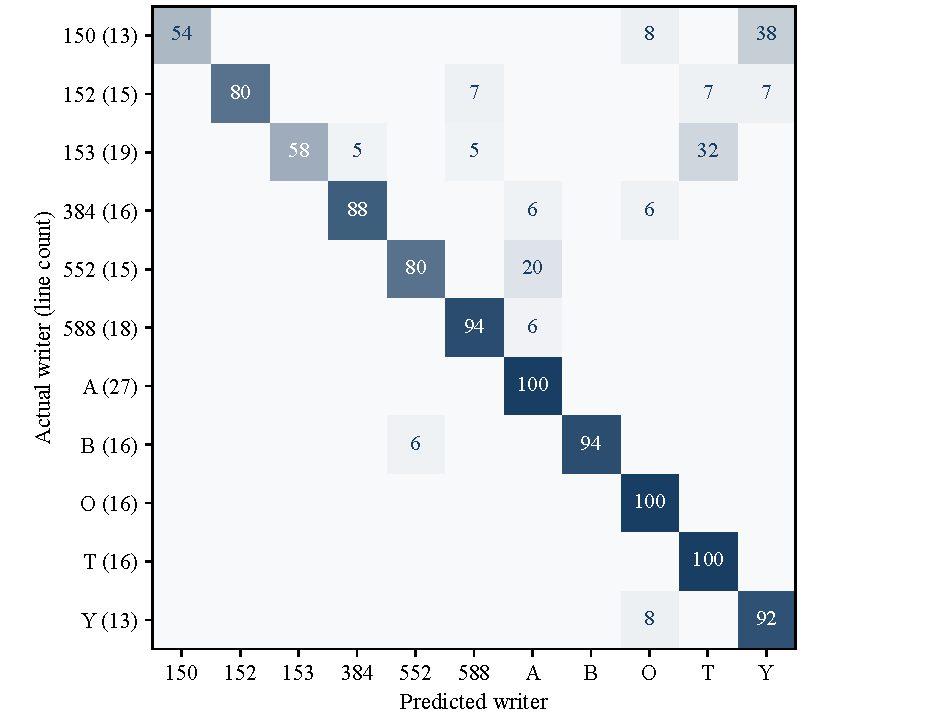
\includegraphics[width=\linewidth]{Figures/rev_physical_confusion.pdf}
\caption{Author predictions on reproduced lines, normalised by actual writer.}
\label{fig:res-reproduced-confusion}\end{figure}

Figure~\ref{fig:res-geometric} gives the geometric result relative to each writer's own variation. Its 100\% reference means equal agreement to the measured natural baseline. Figure~\ref{fig:res-geometric-examples} shows original and robot word crops with their registered skeletons. Appendix~\ref{app:res-geometric} gives the supporting writer averages and further original-to-reproduced examples. The complete crop banks and individual scores remain in the accompanying measurement archive.
\begin{figure}[H]\centering
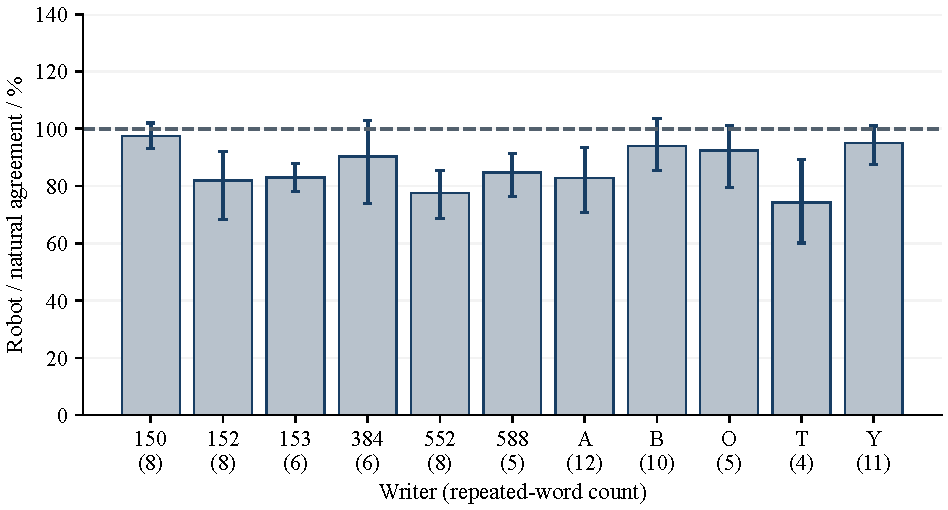
\includegraphics[width=\linewidth]{Figures/rev_geometric_baseline.pdf}
\caption{Geometric agreement relative to natural writing. Counts are repeated words.}
\label{fig:res-geometric}\end{figure}
\begin{figure}[H]\centering
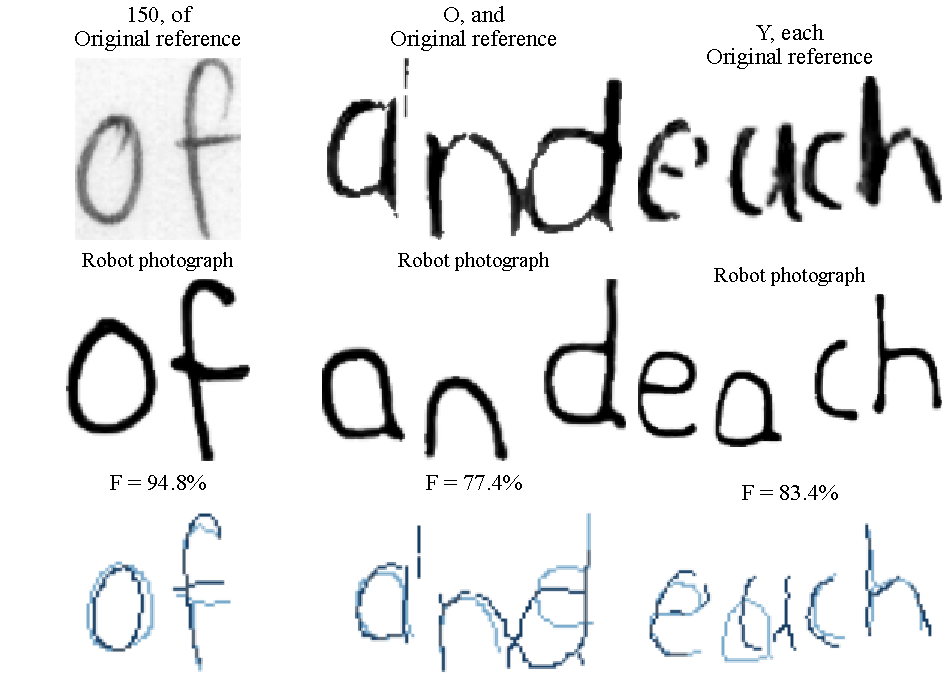
\includegraphics[width=\linewidth]{Figures/rev_geometric_examples.pdf}
\caption{Measured word examples. Dark blue is original, light blue reproduced, grey overlap.}
\label{fig:res-geometric-examples}\end{figure}
\resstep{Observations}
Character scores range from 60.97\% to 97.01\%. Geometric agreement relative to natural writing ranges from 74.26\% to 97.47\% using ordinary reference averages. Twenty-five of 166 eligible source-passage words lack an exact reference. A further 58 of the 141 comparable words lack cross-page repeats for a natural baseline.
\resstep{Statistical analysis}
The 159/184 writer decisions have a descriptive 95\% Wilson interval of 80.7\% to 90.6\%. Figure~\ref{fig:res-geometric} uses 10\,000 paired word-type resamples within the fixed writers and reference banks. The equal-writer range is 83.65\% to 89.65\%. The existing closest-reference sensitivity check gives 87.89\%, compared with the ordinary-reference mean of 86.68\%. The baseline subset contains shorter words than the full geometric population.
\FloatBarrier

\reportqt{qt:r2}{Reading handwritten content and identifying its writer (R2)}

\resstep{Objectives of the test or experiment}

Evaluate reading and writer identification separately against 95\%, using the recorded validation partitions.



\resstep{Equipment used}

Saved IAM and personal line images, reference transcripts, selected checkpoints and the scoring tools. This experiment does not require gantry movement.



\resstep{Test setup and experimental parameters}

The reader population has 976 public validation lines (42\,072 characters) and 100 photographed lines (3\,675 characters). The writer population has 156 lines, using held-out IAM pages and a seeded personal-line split. Personal validation can share page backgrounds with training. These are validation results because checkpoint selection may have used the same split.



\resstep{Steps followed in the test or experiment}

Check the corpus partitions, read each line with greedy CTC decoding, classify the normalised writer crop and retain the edits, reference counts and predictions. Aggregate the reader populations and writer confusion counts separately.



\resstep{Results or measurements}

Table~\ref{tab:res-r2-reader} reports 94.06\% pooled character accuracy for the selected joint reader. The scratch comparison reaches 94.39\% on the same 1\,076 lines. The training-route comparison is in Table~\ref{tab:dis-training}. Table~\ref{tab:app-reader-breakdown} retains the individual personal-writer scores.

\begin{table}[H]\centering\small

\begin{tabular}{lrrrr}\toprule

Population & Lines & Characters & Joint / \% & Scratch / \%\\\midrule

IAM validation & 976 & 42072 & 94.12 & 94.39\\

Personal validation & 100 & 3675 & 93.33 & 94.42\\

Pooled & 1076 & 45747 & 94.06 & 94.39\\\bottomrule

\end{tabular}

\caption{Reader character accuracy on validation lines.}\label{tab:res-r2-reader}

\end{table}



The writer model correctly identifies 153/156 lines (98.08\%) and all eleven pooled writer groups. Figure~\ref{fig:res-holdout} shows the row-normalised predictions, with actual line counts beside each writer. The only three errors are predictions of Y.

\begin{figure}[H]\centering

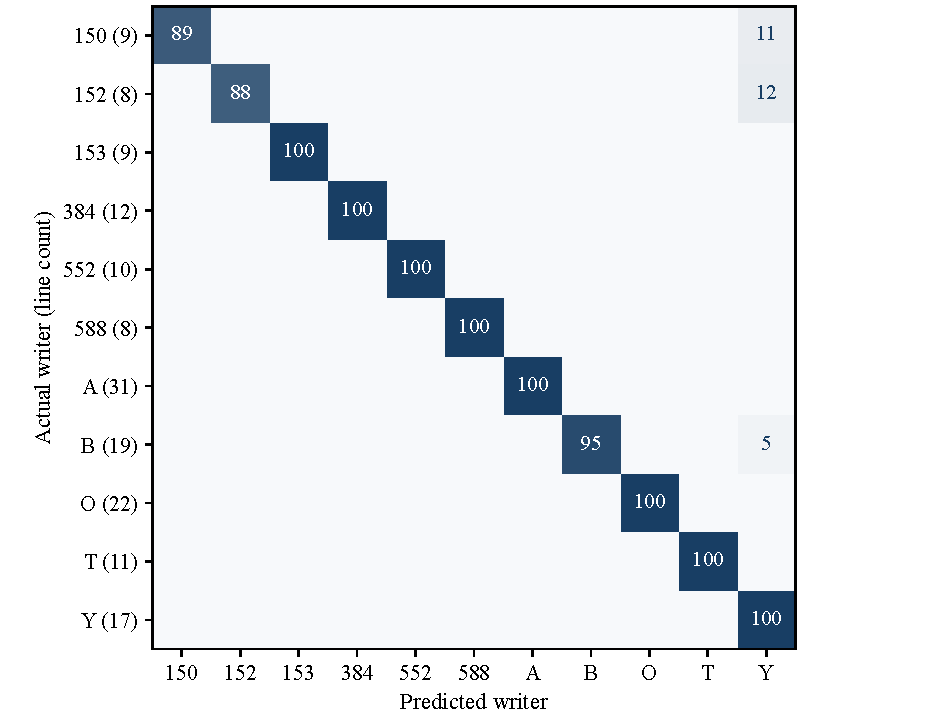
\includegraphics[width=\linewidth]{Figures/rev_validation_confusion.pdf}

\caption{Writer validation predictions, row percentages.}\label{fig:res-holdout}\label{fig:app-validation-confusion}

\end{figure}



\resstep{Observations}

The writer point estimate exceeds target by 3.08 percentage points. The selected reader is 0.94 points below target and recovers 221 complete lines without edits. One incorrect writer prediction has 83.8\% confidence, showing that a high posterior alone cannot guarantee identity.



\resstep{Statistical analysis}

The writer Wilson interval is 94.5\% to 99.3\%. The result demonstrates a point estimate above 95\%, with a stronger pooled decision across the available lines. Character accuracy is an edit-distance ratio, so a binomial interval on individual characters is not assigned.



\FloatBarrier

\reportqt{qt:r3}{Time to reproduce digital text on paper (R3)}
\resstep{Objectives of the test or experiment}
Test whether a completed request containing $x$ characters takes at most $4x$ seconds.
\resstep{Equipment used}
ODROID N2+, gantry, request timer and preserved execution log.
\resstep{Test setup and experimental parameters}
Retain positive-character drawing requests with explicit program-end confirmation. The total includes generation and physical drawing. Stopped jobs and commissioning shapes are excluded.
\resstep{Steps followed in the test or experiment}
Associate each timing record with its completion marker, divide total time by character count and group the retained records by request length.
\resstep{Results or measurements}
Table~\ref{tab:res-r3-confirmed} gives the completed requests. Figure~\ref{fig:res-r3} shows every observation and the measured range at each length. All 25 complete records are in Appendix~\ref{app:res-speed}.
\begin{table}[H]\centering\small
\begin{tabular}{rrrrr}\toprule
\textbf{Characters} & \textbf{Records} & \textbf{Allowance / s} & \textbf{Worst total / s} & \textbf{Worst / s per char}\\\midrule
43 & 9 & 172 & 166.61 & 3.875\\
75 & 1 & 300 & 188.60 & 2.515\\
82 & 3 & 328 & 260.33 & 3.175\\
91 & 2 & 364 & 222.63 & 2.446\\
132 & 1 & 528 & 277.90 & 2.105\\
378 & 9 & 1512 & 1085.01 & 2.870\\
\bottomrule\end{tabular}
\caption{Completed ODROID reproduction jobs by text length.}\label{tab:res-r3-confirmed}
\end{table}

\begin{figure}[H]\centering
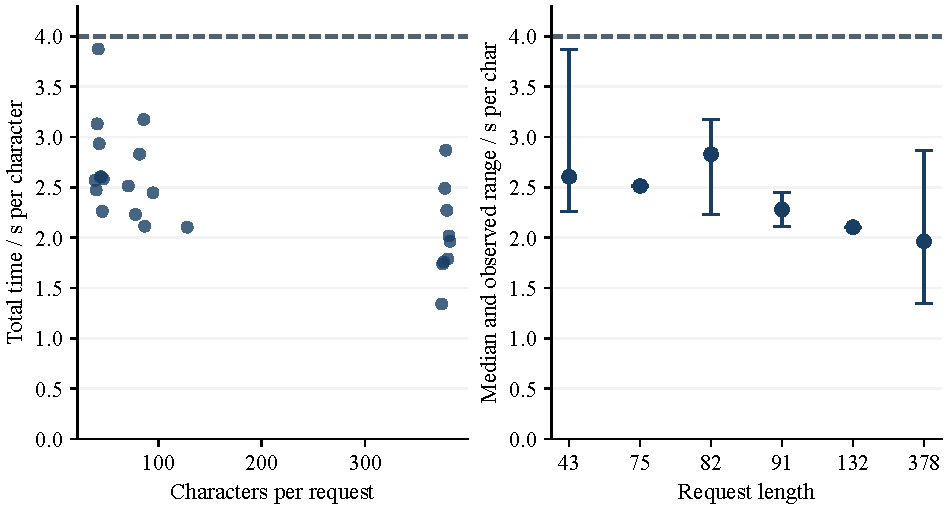
\includegraphics[width=\linewidth]{Figures/rev_reproduction_times.pdf}
\caption{Completed reproduction requests and observed timing ranges.}
\label{fig:res-r3}\end{figure}
\resstep{Observations}
All 25 requests are below 4 s per character. The largest value is $166.61/43=3.875$ s per character. Nine 378-character requests take 507.57 to 1085.01 s.
\resstep{Statistical analysis}
There are one to nine observations at each of six lengths, from 43 to 378 characters. The all-pass fraction has a descriptive Wilson interval of 86.7\% to 100\%. The records do not sample all possible text and path combinations.
\FloatBarrier

\reportqt{qt:r4}{Time to decode a photographed page and identify its writer (R4)}
\resstep{Objectives of the test or experiment}
Compare complete embedded classification with the allowance $2+0.025x$ seconds.
\resstep{Equipment used}
ODROID N2+, request-stage timer and preserved classification log. The laptop records use Windows 11, an Intel Family 6 Model 126 processor with eight logical cores, Python 3.14.3 and NumPy 2.4.3. A separate network benchmark compares sequential numerical inference with batched library modules.
\resstep{Test setup and experimental parameters}
The two embedded records contain 500 characters over 16 lines and 982 over 22 lines. The timer includes loading, conditioning, segmentation, cropping and both networks. Camera acquisition is outside this boundary. The laptop experiment contains thirteen photographed pages, each timed three times. L1 to L8 are writer Y pages and L9 to L13 are writer B pages.
\resstep{Steps followed in the test or experiment}
Read the complete totals and stage times, calculate the character-dependent allowances and compare the measured and allowed values.
\resstep{Results or measurements}
Figure~\ref{fig:res-r4} shows the measured stages and complete totals. Table~\ref{tab:res-r4-total} gives the numerical comparison. Appendix~\ref{app:res-classification-time} retains the recorded stages. Supporting acceleration records remain in the accompanying measurement archive.
\begin{table}[H]\centering\small
\begin{tabular}{rrrrr}\toprule
Characters & Measured / s & Allowed / s & Overrun / s & Measured / allowed\\\midrule
500 & 46.26 & 14.50 & 31.76 & 3.19\\
982 & 55.49 & 26.55 & 28.94 & 2.09\\\bottomrule
\end{tabular}
\caption{Embedded classification totals.}\label{tab:res-r4-total}
\end{table}
\begin{figure}[H]\centering
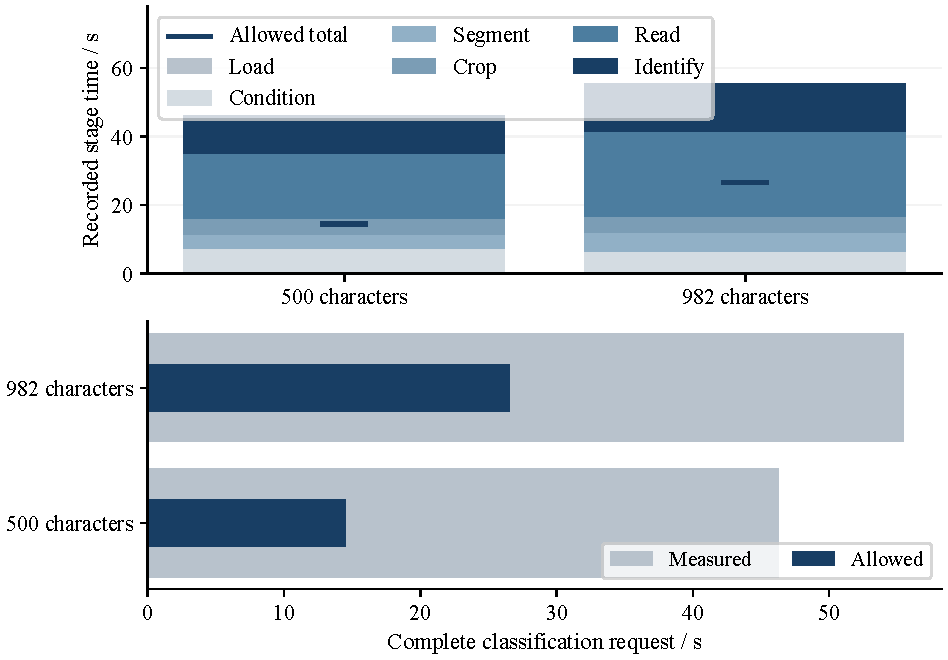
\includegraphics[width=\linewidth]{Figures/rev_classification_times.pdf}
\caption{Recorded classification stages and time allowances.}
\label{fig:res-r4}\end{figure}
The laptop measurements in Table~\ref{tab:res-laptop-times} separate text recognition, author identification and image preparation. Each total is the mean of three recorded requests. All thirteen page means exceed their complete-request allowances.
\begin{table}[H]\centering\small
\begin{tabular}{lrrrrrr}\toprule
Page & Characters & Image / s & Text / s & Author / s & Total / s & Limit / s\\\midrule
L1 & 976 & 34.77 & 7.77 & 5.93 & 48.48 & 26.40\\
L2 & 1168 & 28.94 & 8.44 & 6.60 & 43.99 & 31.20\\
L3 & 1291 & 25.15 & 8.48 & 6.65 & 40.28 & 34.27\\
L4 & 1399 & 30.00 & 8.38 & 7.04 & 45.42 & 36.98\\
L5 & 1677 & 33.45 & 9.60 & 7.66 & 50.71 & 43.93\\
L6 & 1301 & 30.94 & 8.64 & 6.74 & 46.32 & 34.52\\
L7 & 1316 & 31.28 & 8.57 & 6.67 & 46.52 & 34.90\\
L8 & 1388 & 31.71 & 9.38 & 7.43 & 48.52 & 36.70\\
L9 & 1186 & 37.30 & 9.14 & 6.97 & 53.41 & 31.65\\
L10 & 1296 & 57.94 & 15.92 & 11.65 & 85.51 & 34.40\\
L11 & 1262 & 69.84 & 17.36 & 12.87 & 100.06 & 33.55\\
L12 & 1040 & 53.73 & 14.14 & 10.66 & 78.53 & 28.00\\
L13 & 1186 & 53.56 & 14.03 & 11.88 & 79.47 & 31.65\\
\bottomrule\end{tabular}
\caption{Laptop classification times, means of three runs per page. Image includes loading.}\label{tab:res-laptop-times}\end{table}

The existing fourteen-page network benchmark takes 359.8 s sequentially and 130.3 s using batched library modules, a factor of 2.76. Reader output is identical on every evaluated line. Both batching and backend change, so their individual gains and author-label equivalence are not established.

Table~\ref{tab:res-laptop-projection} applies that factor to the combined network stages of selected laptop records while retaining their measured image times. The estimate uses $t_{\rm image}+(t_{\rm text}+t_{\rm author})/2.76$. This would bring L3, L4 and L5 inside their budgets if the factor transfers. L1 remains above its limit because image processing alone takes 34.77 s. These are conditional estimates from a separate benchmark, rather than measured passes.
\begin{table}[H]\centering\small
\begin{tabular}{lrrrrl}\toprule
Page & Characters & Recorded / s & Limit / s & Estimated / s & Estimate\\\midrule
L1 & 976 & 48.48 & 26.40 & 39.74 & Above limit\\
L3 & 1291 & 40.28 & 34.27 & 30.63 & Within limit\\
L4 & 1399 & 45.42 & 36.98 & 35.59 & Within limit\\
L5 & 1677 & 50.71 & 43.93 & 39.70 & Within limit\\
\bottomrule\end{tabular}
\caption{Conditional laptop totals with unchanged image time and 2.76 times faster networks.}\label{tab:res-laptop-projection}\end{table}

\resstep{Observations}
Both ODROID requests and all thirteen laptop page means exceed their allowances. Networks account for 67.6\% of the combined ODROID time. The laptop records also show substantial image-processing cost, so network acceleration alone cannot bring every page within specification.
\resstep{Statistical analysis}
The laptop set has three repetitions per page and the embedded log has two complete requests. The library benchmark measures a network gain on fourteen saved pages. Its transfer to other requests or the ODROID is a projection. Halving image resolution is not an equivalent remedy, since the recorded trial lost lines and changed the recognised text.
\FloatBarrier

\reportqt{qt:r5}{Gantry dimensional accuracy and repeated geometric samples (R5)}
\resstep{Objectives of the test or experiment}
Compare repeated square and triangle feature lengths with the 0.5 mm error limit.
\resstep{Equipment used}
Final calibrated gantry, pen, paper and the author's metal non-digital vernier caliper. The instrument model and least count are not recorded.
\resstep{Test setup and experimental parameters}
Ten supplied samples each contain four nominal 100.00 mm square sides, an 80.00 mm triangle base and two nominal 56.57 mm slopes. These give 70 readings. Errors use the supplied two-decimal nominal lengths.
\resstep{Steps followed in the test or experiment}
Measure all seven features on each sample, subtract the nominal length and retain signed errors. Group the readings by feature and sample without treating seven sides of one drawing as seven independent drawings.
\resstep{Results or measurements}
Figure~\ref{fig:res-geometry} contains every signed error, so individual samples can be checked against the limit. Table~\ref{tab:res-gantry-summary} summarises the complete set. Appendix~\ref{app:res-geometry-calculation} retains the feature statistics. All 70 supplied readings remain in the accompanying measurement archive.
\begin{table}[H]\centering\small
\begin{tabular}{lr}
\toprule Recorded quantity & Value\\\midrule
Geometric samples & 10\\
Measured feature lengths & 70\\
Lengths within 0.5 mm & 70/70\\
Mean absolute length error & 0.297 mm\\
RMS length error & 0.327 mm\\
Largest absolute length error & 0.49 mm\\
\bottomrule\end{tabular}
\caption{Ten-sample dimensional summary.}\label{tab:res-gantry-summary}\end{table}

\begin{figure}[H]\centering
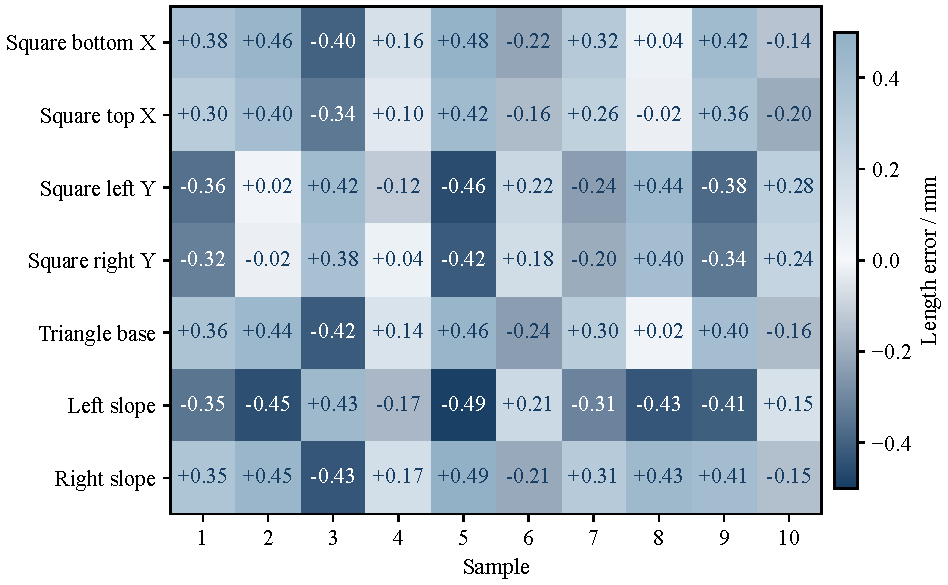
\includegraphics[width=\linewidth]{Figures/rev_gantry_errors.pdf}
\caption{All 70 signed feature-length errors in millimetres.}
\label{fig:res-geometry}\end{figure}
\resstep{Observations}
All 70 reported lengths are within 0.5 mm of nominal. The largest errors are the two triangle slopes in sample 5, at $-0.49$ and $+0.49$ mm. Square-side errors change sign between samples. The supplied measurements describe feature lengths rather than absolute bed coordinates.
\resstep{Statistical analysis}
Each feature has ten readings. Sample standard deviations describe variation among those readings. The minimum observed margin to the limit is 0.01 mm. Measurement uncertainty cannot be assigned from the retained record because caliper resolution and the nib-edge reading convention are unspecified.
\FloatBarrier

\reportqt{qt:r6}{Storage and use of multiple trained styles (R6)}
\resstep{Objectives of the test or experiment}
Check the required minimum of ten stored and usable writer styles.
\resstep{Equipment used}
Writer mapping, stored glyph profiles, generated jobs and fourteen physical output pages.
\resstep{Test setup and experimental parameters}
The evaluated set contains eleven identities. Each must have a nonempty stored glyph mapping and physical output.
\resstep{Steps followed in the test or experiment}
Compare model identities with profile keys and confirm the corresponding reproduced pages.
\resstep{Results or measurements}
All eleven stored styles have physical output, exceeding the required minimum of ten. Appendix~\ref{app:res-inventory} lists their mapping and page counts, followed by the photographed pages.
\resstep{Observations}
The style count exceeds the required minimum by one. Character coverage differs between profiles.
\resstep{Statistical analysis}
This is a complete inventory of the evaluated profiles, rather than a sample estimate.

\subsubsection{Qualification under the proposal's field conditions}
\label{sec:res-conditions}
The recorded tests use the fixed indoor capture and gantry arrangement. The capture variations already shown in Design extend the visual evidence. No calibrated illuminance or vibration series is assigned to these results.
\FloatBarrier

\endgroup
